%%
\documentclass[format=draft,language=chinese,category=SDN]{hustreport}
\hypersetup{
    colorlinks=true,
    linkcolor=blue,
    filecolor=magenta,
    urlcolor=blue
}
\lstset{language=sh,columns=fullflexible,frame=single}
\newcommand{\myparagraph}[1]{\paragraph{#1}\mbox{}\\}
\newcommand{\code}{\texttt}

\title{初赛文档}
\author{\kai{林家军}~~\kai{李英儒}~~\kai{胡云锐}}
\major{计算机科学与技术}
\department{计算机科学与技术学院}
\advisor{\kai{周世伟}}

\abstract{
    这是来自华中科技大学UniqueSDNStudio队伍的初赛文档,于\LaTeX{}编辑而成。

}
\keywords{软件定义网络, SDN, \LaTeX{}, 华中科技大学}


\begin{document}
\nocite{*}

\frontmatter
\maketitle
\makeabstract
\tableofcontents
%\listoffigures
%\listoftables
\mainmatter

\chapter{基础环境}\label{chapter:BaiscEnv}
SDN 的基础环境由 SDN 控制器(Controller)和支持 SDN 的交换机构成
的网络组成,我们在本次比赛中使用 Ryu 作为 SDN 控制器,使用 Mininet 构建
虚拟试验网络。
\section{Ryu}
Ryu is a component-based software defined networking framework.

Ryu是一个基于组件的软件定义网络框架。

Ryu provides software components with well defined API that make it easy for developers to create new network management and control applications. Ryu supports various protocols for managing network devices, such as OpenFlow, Netconf, OF-config, etc. About OpenFlow, Ryu supports fully 1.0, 1.2, 1.3, 1.4 and Nicira Extensions.

Ryu提供了具有良好设计的API结构的软件组件,使得开发者能够更加方便简单地创建新的网络管理控制应用。Ryu支持许多管理网络设备的协议,例如OpenFlow, Netconf, OF-config等。关于Openflow,Ryu支持全部1.0, 1.2, 1.3, 1.4和Nicira扩展。

All of the code is freely available under the Apache 2.0 license. Ryu is fully written in Python.

所有Ryu代码能够在Apache 2.0 许可下自由地获取。 Ryu全部由Python写成。

\section{Mininet}
Mininet 是由一些虚拟的终端节点(end-hosts)、交换机、路由器连接而成的一个网络仿真器,它采用轻量级的虚拟化技术使得系统可以和真实网络相媲美。它可以很方便的创建一个支持 SDN 的网络,有了这个网络,就可以灵活的为网络添加新的功能并进行相关测试。

\chapter{参赛情况}\label{chapter:Situation}


\section{竞赛组织及参与情况}
本次竞赛的组织活动由校教务处发起,在全校范围内自主报名参加。联创团队的参赛队伍共有两支。本组名为UniqueSDNStudio,由三名大二本科生组成,并安排有一位研究生作为指导老师。在参赛过程中,每周每人大约工作时间 40 小时且每周六进行一次讨论总结上周情况并对下周进行科学严谨的安排,为保证作品按时完成我们建立了邮件组与在线讨论平台,同一管理协调。
\section{参赛队伍构成}
\subsection{联创团队}
联创团队$(Unique Studio)$于 2000 年 6 月创建于华中科技大学,是 $Teamwork$ 和
 $Creation$ 为团队核心的学生团队。团队名称来源于“联众人之智”必能“创非凡之事”的信念
。联创团队建立了一个自主的精英学生平台,在这个平台上学生自我管理,通过这个平台激发无限的潜力和创意。
自成立到现在,联创团队已参加微软创新杯 11 次并 8 次进入全球总决赛拿下包括全球冠军等优秀成绩。
除此之外,联创团队也多次参加各种大小型比赛并取得了骄人的成绩,并与$MICROSOFT$\texttrademark、$CSDN$\texttrademark 等公司保持着非常好的合作关系,同时加入微软中国组织的创新联盟。
联创团队多年的发展积累了独特的文化和运作机制,同时跟踪技术发展的最前沿,这使得联创团队在华科乃至全国高校中独树一帜。
\subsection{指导老师}
\kai{周世伟}

\textbf{华中科技大学} 2010级本科生,2014 级研究生,现就读于光电与电子信息学院光电信息工程专业。华中科技大学联创团队 IT 组和嵌入式组成员。曾 2 次获得国家奖学金。参与 微软创新杯$Imagine~Cup\texttrademark$ $IT~Challenge\textregistered$ 比赛,并进入中国区总决赛。曾获得
中国区第一届 $RDMA\textregistered$ 比赛一等奖。目前已获得华中科技大学保研资格。
\href{http://zhoushiwei1992.blog.163.com}{周世伟个人博客。}
\subsection{参赛队员}
\kai{林家军}

\textbf{华中科技大学} 2013 级本科生,现就读于计算机科学与技术学院计算机科学与技术专业。华中科技大学联创团队 IT 组成员。

\kai{李英儒}

\textbf{华中科技大学} 2013 级本科生,现就读于计算机科学与技术学院计算机科学与技术专业。华中科技大学联创团队 IT 组成员。

\kai{胡云锐}

\textbf{华中科技大学} 2013 级本科生,现就读于计算机科学与技术专业。
华中科技大学联创团队 IT 组成员,主要进行网络通讯、大数据方面的研究。

\chapter{初赛题目}\label{chapter:Questions}


\section{第一题:基础题}\label{sec:Q1}
\subsection{第1小题:简单网络}\label{sec:Q1_1}

\begin{figure}[!h] \centering
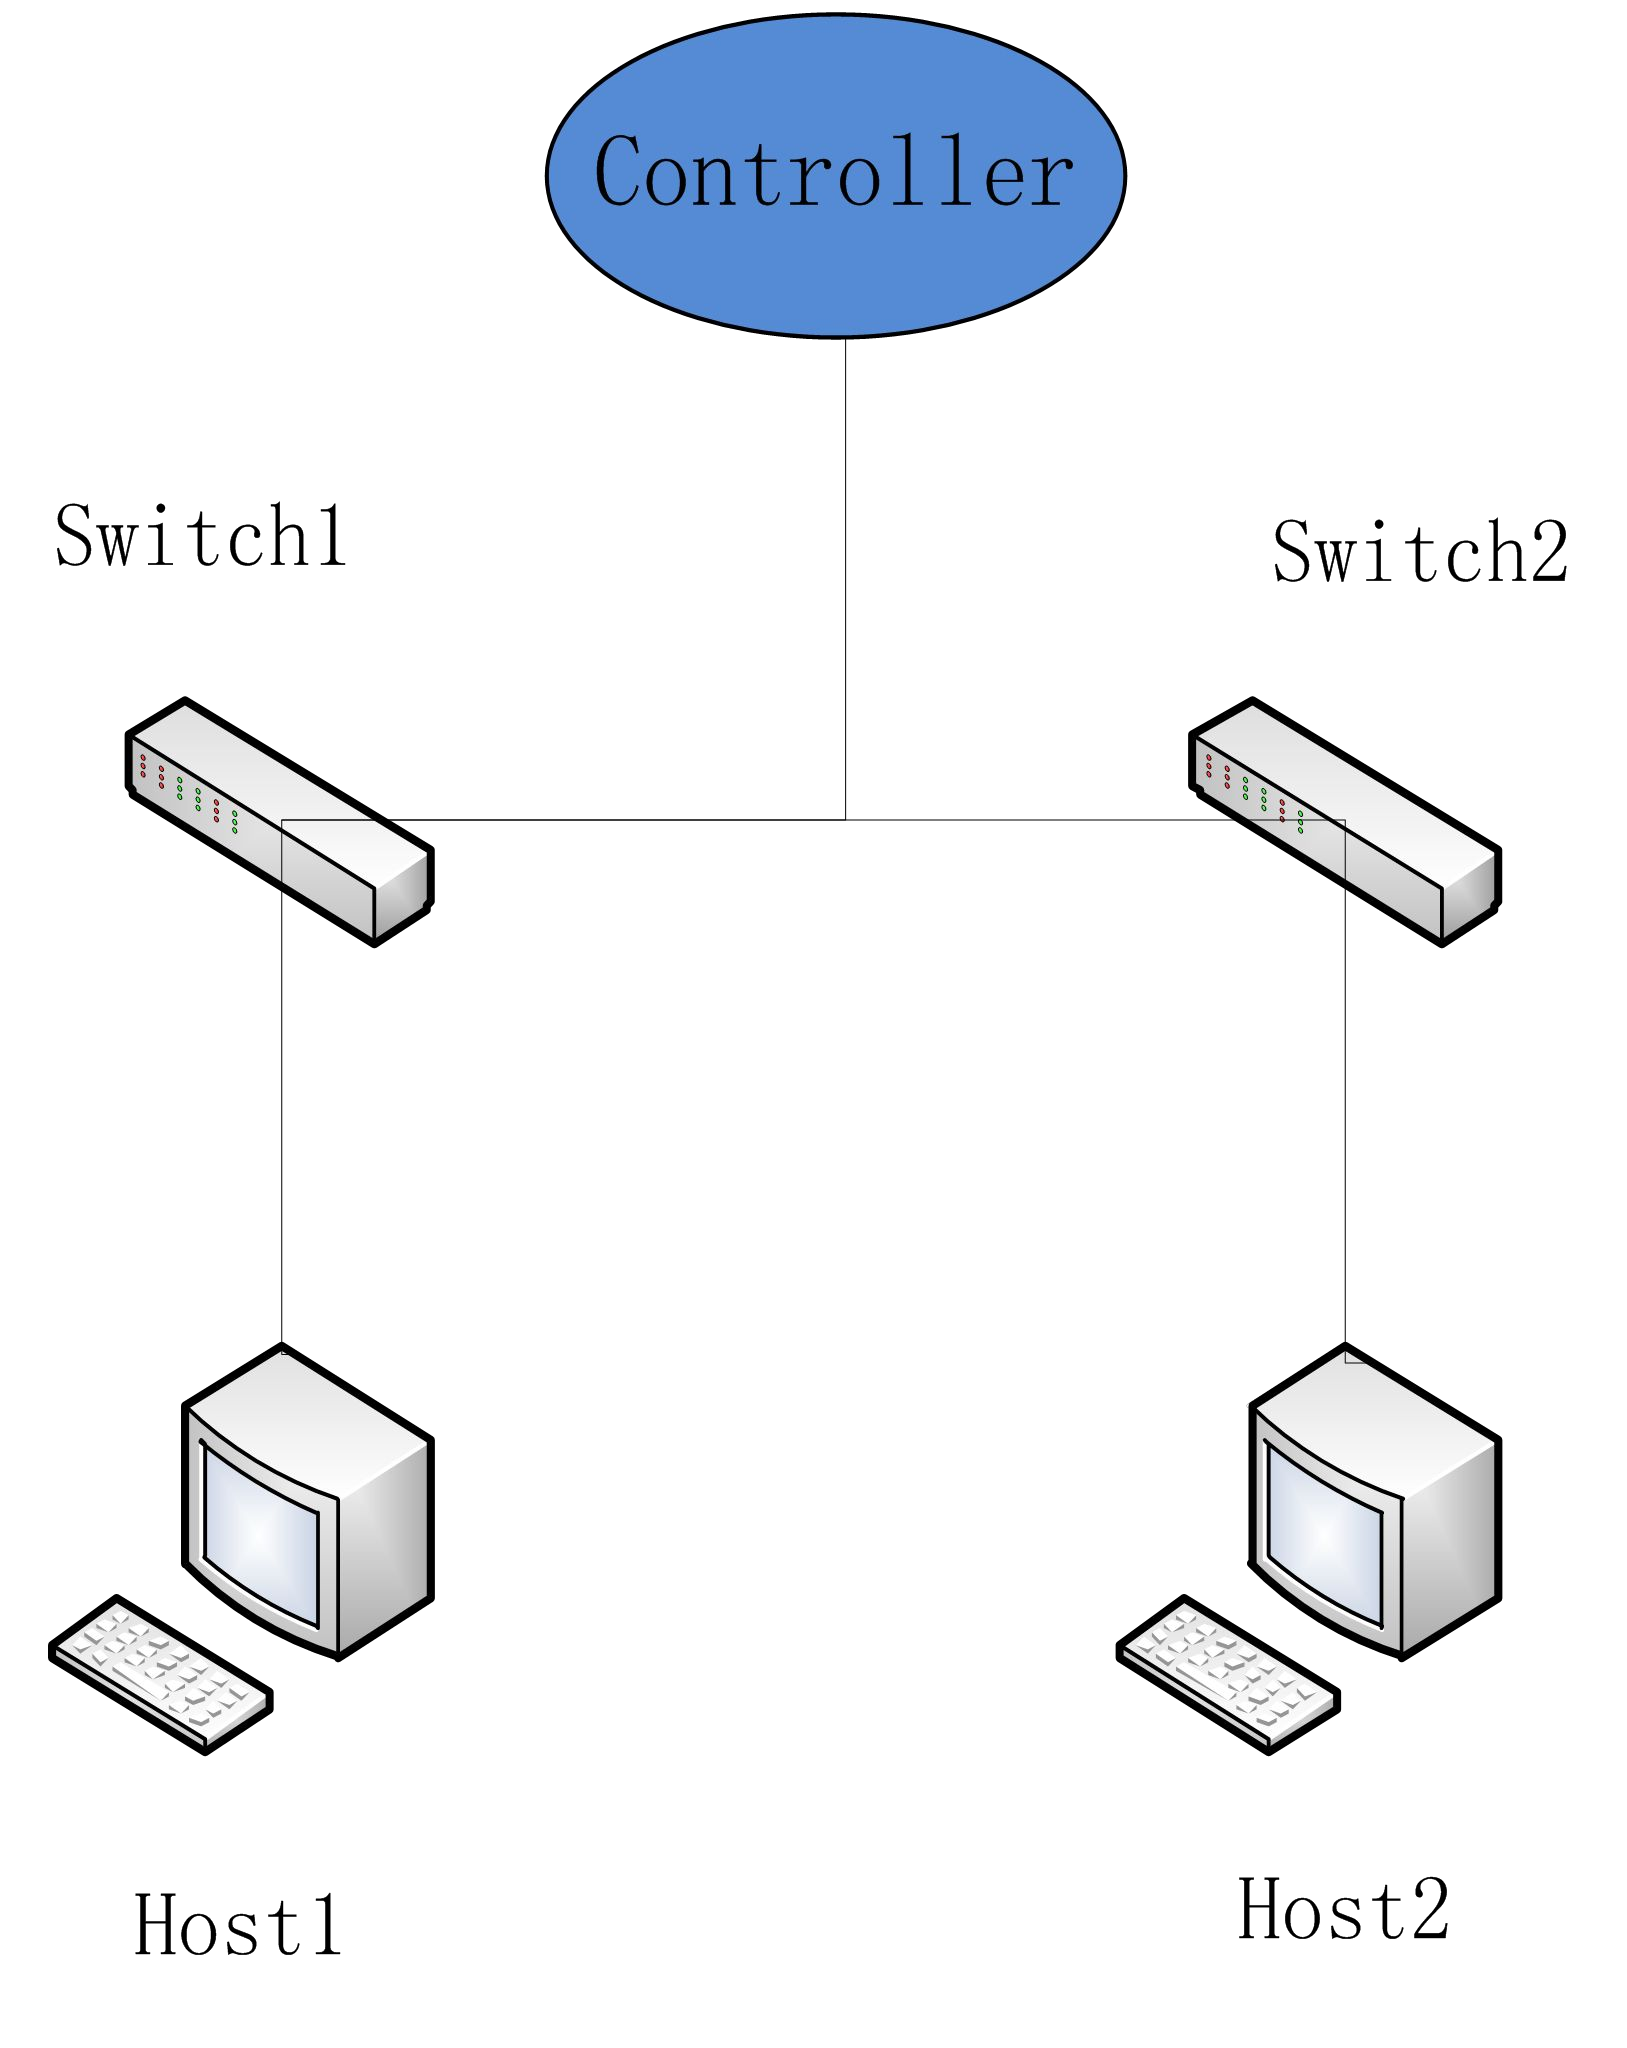
\includegraphics[width=.618\textwidth]{fig/1_1-0.png}
\caption{第一题第1小题:简单网络}\label{fig:Q1_1-0}
\end{figure}

\myparagraph{网络环境要求}

要求搭建的网络环境如图 1 所示(Controller 表示控制器, switch 表示交换机, host表示主机)。控制器可以自主选择,例如各种开源的控制器(Floodlight、Ryu、
Nox、Beacon、Trema、OpenDaylight 等)。拓扑中各网络部件既可以是仿真环境实现(例如 mininet, OpenvSwtich 等),有条件的队伍也可以通过物理设备实现,
各种方案不影响评分。试题中每道题都遵循这些要求,不再说明。

\myparagraph{操作要求}

1.先使 Host1 可以 ping 通 Host2,Host2 也可以 ping 通 Host1。

2.然后对流表进行操作,使 Host1 不能 ping 通 Host2, Host2 也不能 ping 通 Host1。

\myparagraph{方法描述}

利用 mininet 创建虚拟环境,在虚拟交换机上直接修改流表。

\myparagraph{实验步骤}

1. 打开 mininet 创建一个拓扑,它包含一个交换机和两个主机。命令如下:

\begin{lstlisting}
mn --topo single,2
\end{lstlisting}

2. 在 mininet CLI 中检查环境,确认流表为空。

3. 执行如下两条命令,添加流表,使两个虚拟主机可以通信。

\begin{lstlisting}
s1 ovs-ofctl add-flow "s1" in_port=1,action=output:2
s1 ovs-ofctl add-flow "s1" in_port=2,action=output:1
\end{lstlisting}

4. 执行 \code{pingall} 检查网络环境,结果见\autoref{fig:Q1_1-1},h1 与 h2 可以正常通信。

\begin{figure}[!h]
\centering
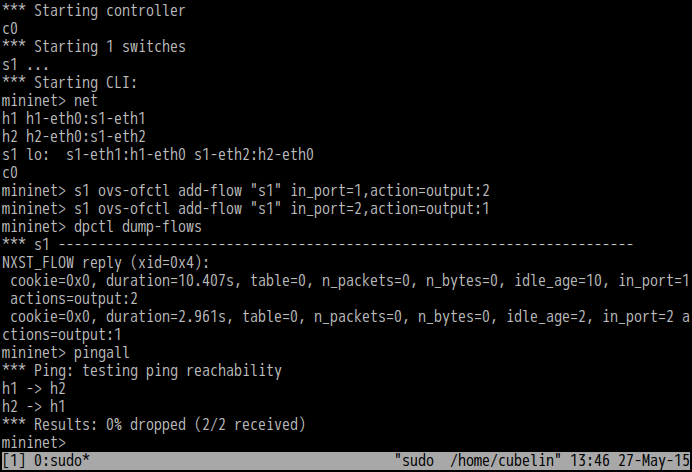
\includegraphics[width=.618\textwidth]{fig/1_1-1.png}
\caption{检查虚拟网络环境}\label{fig:Q1_1-1}
\end{figure}

5. 执行如下两条命令,删除添加的流表。

\begin{lstlisting}
s1 ovs-ofctl del-flows "s1" in_port=1
s1 ovs-ofctl del-flows "s1" in_port=2
\end{lstlisting}

6. 执行 \code{pingall} 再次检查网络环境,结果见\autoref{fig:Q1_1-2},h1 与 h2 无法正常通信。

\begin{figure}[!h]
\centering
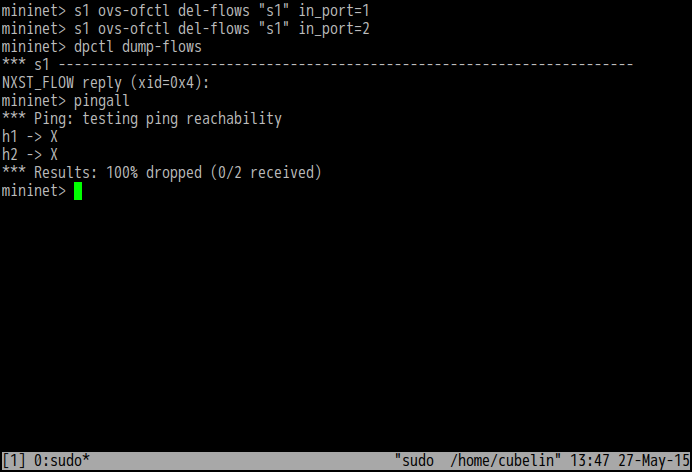
\includegraphics[width=.618\textwidth]{fig/1_1-2.png}
\caption{删除流表后检查虚拟网络环境}\label{fig:Q1_1-2}
\end{figure}

\myparagraph{实验结果}

通过修改交换机的流表,先后成功实现虚拟主机 h1 与 h2 能互相 ping 通,与 ping 不通。

\clearpage

\subsection{第2小题:访问限制}\label{sec:Q1_2}

\begin{figure}[!h]
\centering
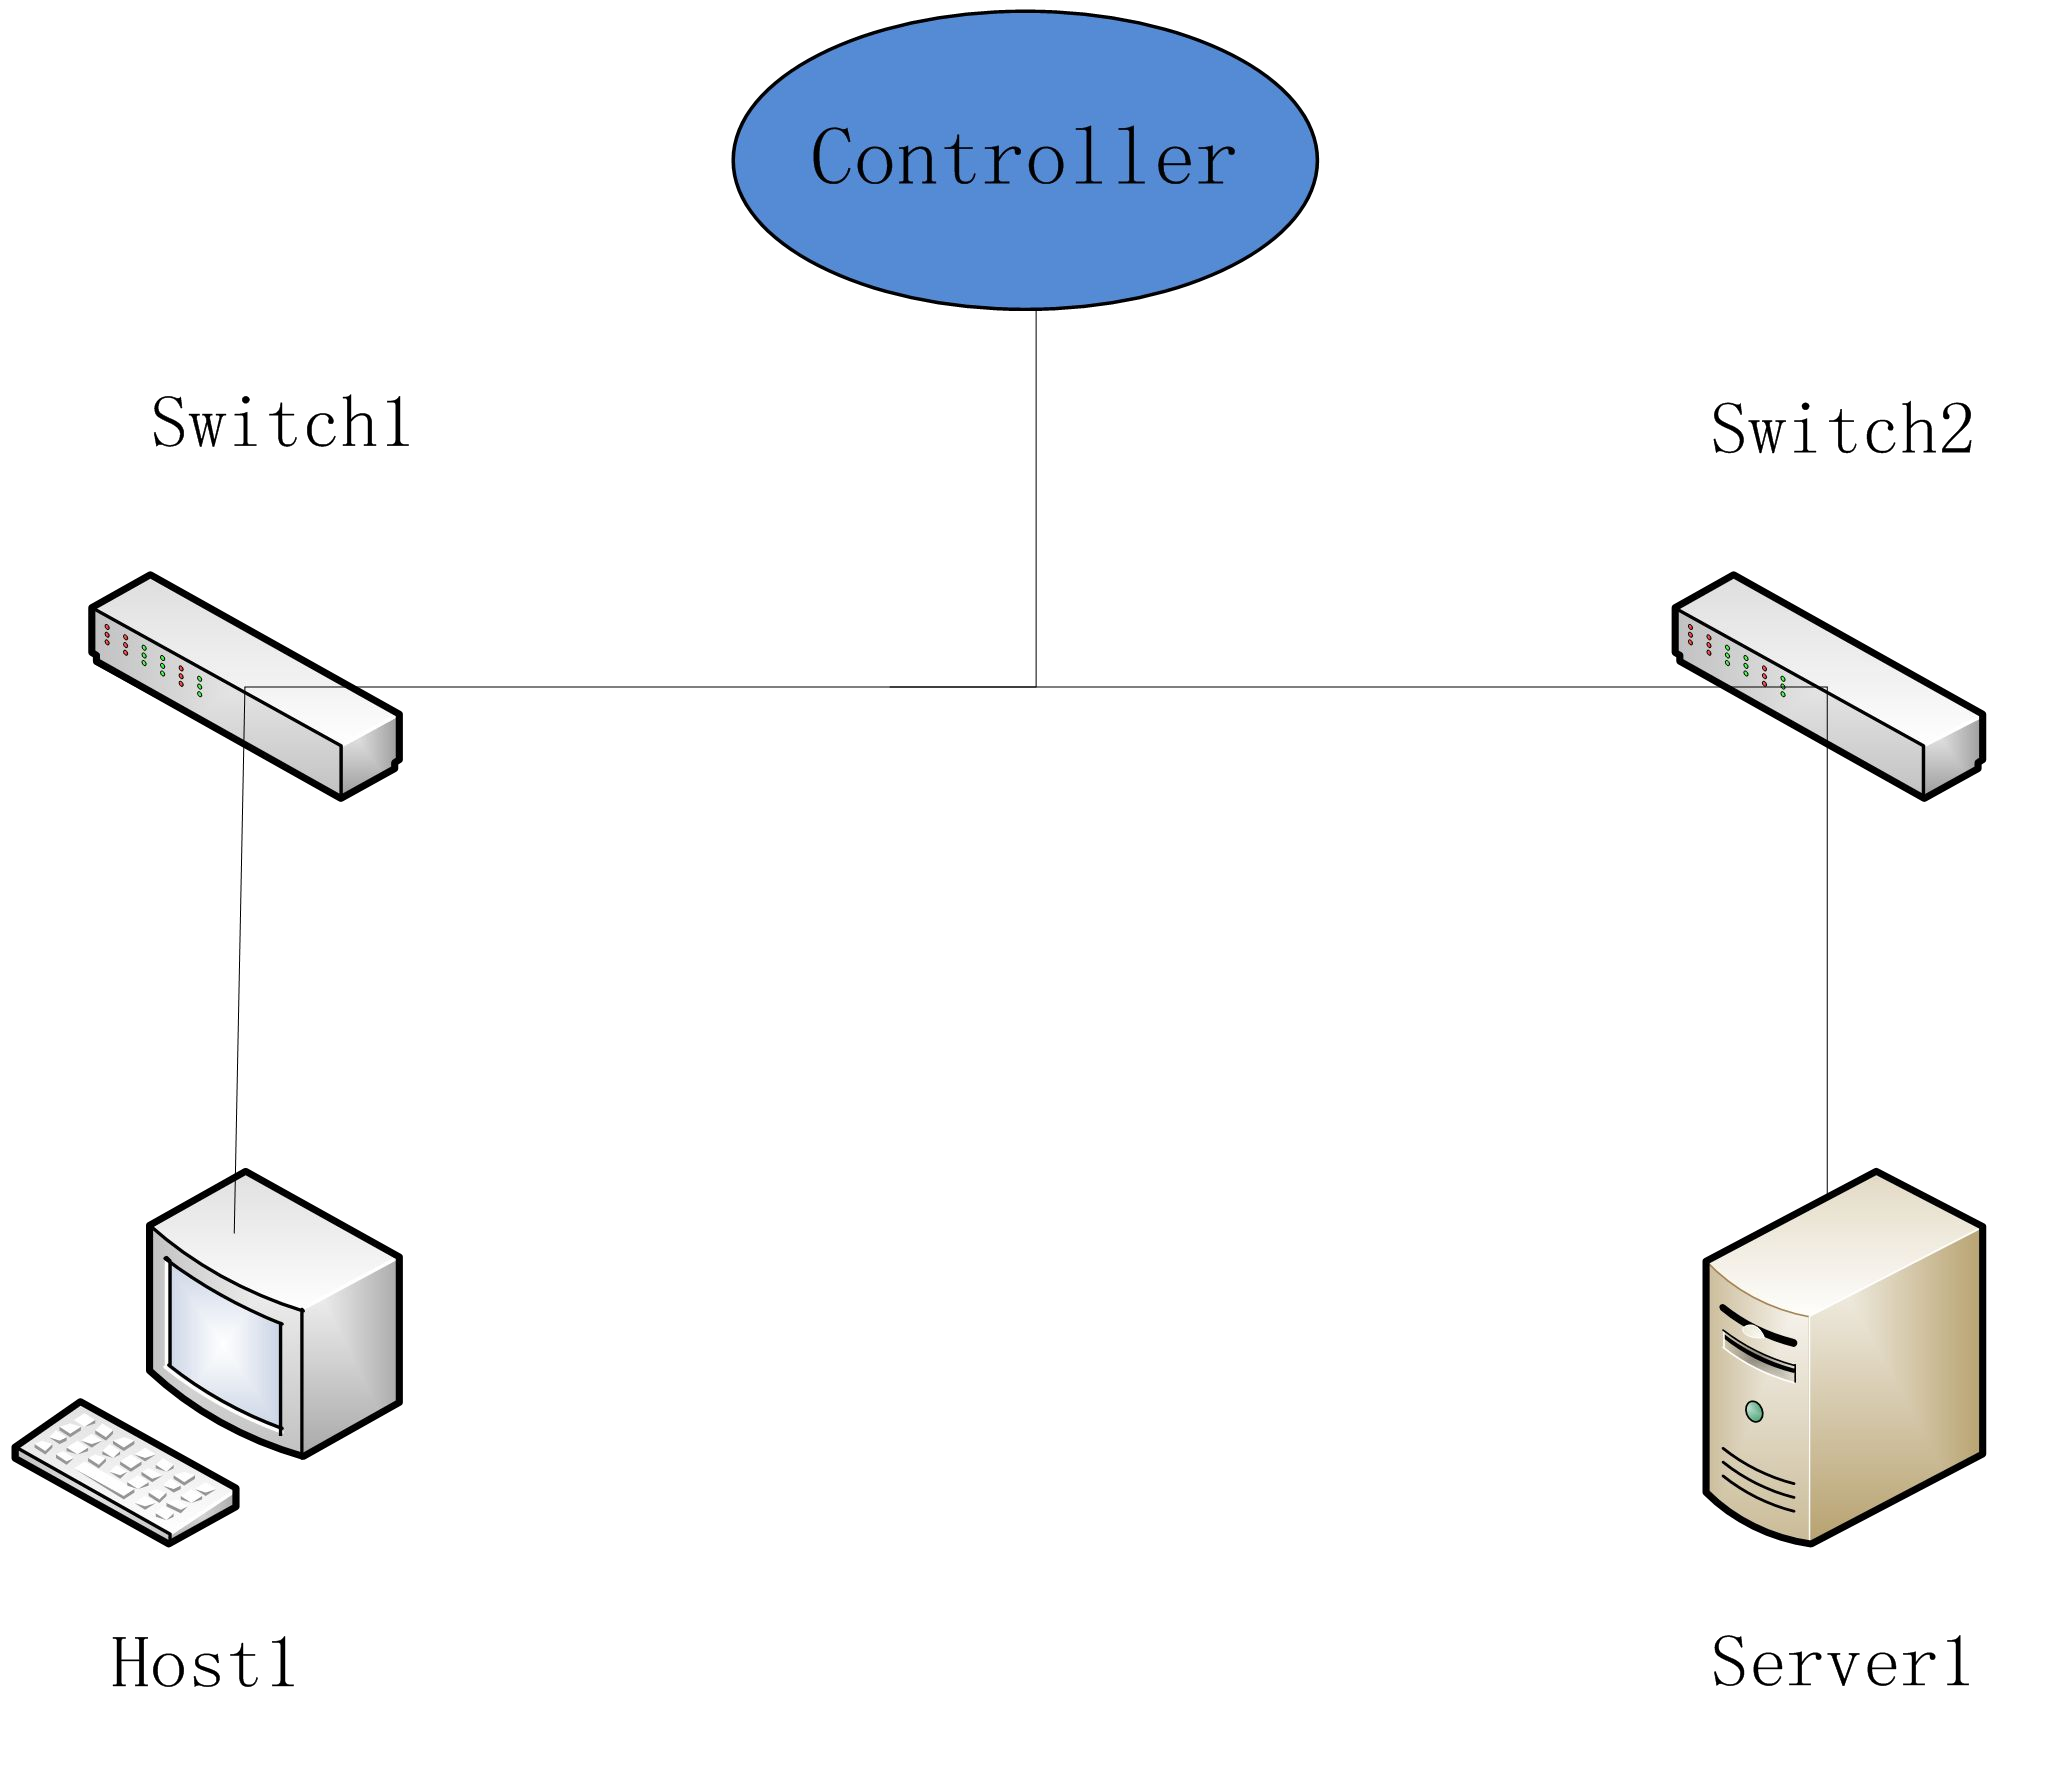
\includegraphics[width=.618\textwidth]{fig/1_2-0.png}
\caption{第一题第1小题:访问限制}\label{fig:Q1_2-0}
\end{figure}

\myparagraph{网络环境要求}

设有一台 PC 机(Host1),一台 Web 服务器(Server1)提供简单的静态网页访问服务,如图 2 所示。(PC 机、Web 服务器、交换机、控制器可以选择物理设备或者虚拟设备实现)

\myparagraph{操作要求}

1.先使得 PC 机访问服务器成功(即看到服务器的网页)。

2.限制该 PC 机一定时间(比如一分钟)内再次访问服务器。限制时间过后,PC机可以成功访问服务器。

\myparagraph{方法描述}

拓扑环境如\autoref{fig:Q1_2-0},其中 Host1 为 h1,Server1 为 h2。

为了一般性,我们编写了第三方 Ryu Controller App, 接收交换机连接 Controller 时发来的 Feature message, 并为交换机添加默认流表。与第一小题类似的,每个交换机各有两个 flow entry 保证主机 h1 和 h2 的正常通信。

s2 中有一个额外的 flow entry,实现将 h1 发来的 TCP 包,在送出交换机 2 号端口的同时复制一份送给 Controller。Controller分析后,检查此包来源的 mac 是否在白名单中,并判断此包是否为 TCP 三次握手包 ($ACK \leq 1$)。若此包并不是 TCP 三次握手包,而且其来源 mac 地址不在白名单中,Controller 将立即为交换机添加一个带有 60 秒 hard\_timeout 的 flow entry,丢弃所有来自此 mac 并且目的 mac 地址是主机 h2 的 http 包,阻断其请求,但是仍可接收来自 h2 的返回,之后将此 mac 加入白名单。

60 秒过后,此 flow entry 过期,而来源 mac 已在白名单中,此后的请求将不会被阻止。

流程伪代码如下:

\begin{algorithm}[H]
	\SetAlgoLined
	\textbf{Initial}  $Ryu~Controller~\&~White~List = \varnothing$ \;\label{alg_line:Q1_2DataPlane}
	\textbf{DATA PLANE}[Hardware Layer]\;
	\While{Flowtable \textbf{Match} $TCP\_packet$ from h1}{
	\textbf{Send} $TCP\_packet$ to $port~2$ and its copy to $Ryu Controller$ \;
	}

	\textbf{CONTROL PLANE}[Software Layer]\;
	\While{\textbf{Recieve} $TCP\_packet$}{
        \If{$TCP\_packet.source\_mac \notin White List$ \textbf{and} $TCP\_packet.ACK > 1$}{

				\textbf{Send} Flow Entry with $hard\_timeout=60$ to \textbf{Drop} $HTTP~Package$ from $TCP\_packet.source\_mac$ to $h2.mac$\;

				$White~List \Leftarrow White~List \cup \{TCP\_packet.source\_mac\}$ \;
		}
	}
	\caption{Visiting Constraints using SDN}\label{alg:Q1_2}
\end{algorithm}

\myparagraph{实验步骤}

1. 进入附件 1.1 目录,执行如下命令,其中 setup\_network.py 用于搭建虚拟网络环境,执行该脚本需要 root 权限。1\_2.py 是我们编写的 Ryu Controller App。

\begin{lstlisting}
python2 setup_network.py
ryu-manager 1_2.py
\end{lstlisting}

交换机连接 Controller 后,会往 Controller 发送 Feature message,以下代码将发挥作用。

\begin{lstlisting}[language=python]
...
    @set_ev_cls(ofp_event.EventOFPSwitchFeatures, CONFIG_DISPATCHER)
    def switch_feature_handler(self, ev):
        datapath = ev.msg.datapath
        ofproto = datapath.ofproto
        parser = datapath.ofproto_parser
        dpid = datapath.id

        self.logger.info("Switch %d connected, adding flow entries.", dpid)
        match = parser.OFPMatch(in_port=1)
        actions = [parser.OFPActionOutput(2, ofproto.OFPCML_NO_BUFFER)]
        # Flow entry match structure: priority=0,in_port=1 actions=output:2
        self.add_flow(datapath, 0, match, actions)

        match = parser.OFPMatch(in_port=2)
        actions = [parser.OFPActionOutput(1, ofproto.OFPCML_NO_BUFFER)]
        # Flow entry match structure: priority=0,in_port=2 actions=output:1
        self.add_flow(datapath, 0, match, actions)

        if dpid == 2:
            match = parser.OFPMatch(in_port=1, eth_type=PROTO_IP,
                                    ip_proto=PROTO_TCP, tcp_dst=80)
            actions = [parser.OFPActionOutput(2, ofproto.OFPCML_NO_BUFFER),
                       parser.OFPActionOutput(ofproto.OFPP_CONTROLLER,
                                              ofproto.OFPCML_NO_BUFFER)]
            # Flow entry match structure:
            # priority=1,tcp,in_port=1,tp_dst=80
            # actions=output:2,CONTROLLER:65535
            self.add_flow(datapath, 1, match, actions)

...
\end{lstlisting}

2. 在 mininet CLI 中检查网络环境,结果如\autoref{fig:Q1_2-1}。

3. 在 mininet CLI 中执行 \code{h2 xterm \&},并在打开的 xterm 中执行 \code{python -m HTTPServer 80} 打开 Web 服务器。

4. 回到 mininet CLI 中执行 \code{h1 curl h2}, 得到以下返回
\begin{center}
**this\_is\_the\_web\_page\_of\_problem\_1.2**
\end{center}
一分钟内再次执行 \code{h1 curl h2 -m 10},超时。检查流表,结果如\autoref{fig:Q1_2-2}。

Controller 接受到 PacketIn message 时,以下代码将会发挥作用。

\begin{lstlisting}[language=python]
...
    @set_ev_cls(ofp_event.EventOFPPacketIn, MAIN_DISPATCHER)
    def _packet_in_handler(self, ev):
        msg = ev.msg
        datapath = msg.datapath
        parser = datapath.ofproto_parser
        in_port = msg.match['in_port']
        dpid = datapath.id
        pkt = packet.Packet(msg.data)
        eth = pkt.get_protocols(ethernet.ethernet)[0]
        dst = eth.dst
        src = eth.src
        tcp_p = pkt.get_protocols(tcp.tcp)

        if dpid != 2 or src in self.macs or len(tcp_p) == 0:
            return

        tcp_p = tcp_p[0]
        if tcp_p.ack <= 1:  # TCP three-way handshake and HTTP request
            return

        self.logger.info("First HTTP request from %s, adding flow entry.", src)

        self.macs.append(src)
        actions = []
        match = parser.OFPMatch(in_port=in_port, eth_src=src, eth_dst=dst,
                                eth_type=PROTO_IP, ip_proto=PROTO_TCP,
                                tcp_dst=80)
        # Flow entry match structure:
        # priority=2,tcp,in_port=1,dl_src=xx:xx:xx:xx:xx:xx,
        # dl_dst=xx:xx:xx:xx:xx:xx,tp_dst=80 actions=drop
        self.add_flow(datapath, 2, match, actions, hard_timeout=60)

...
\end{lstlisting}

\global\csname @topnum\endcsname 0 % prevent figures breaking lstlisting

\begin{figure}[!h]
\centering
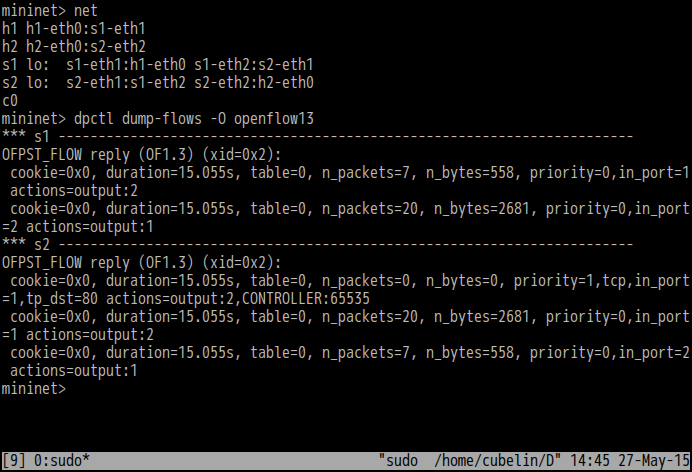
\includegraphics[width=.618\textwidth]{fig/1_2-1.png}
\caption{检查网络环境}\label{fig:Q1_2-1}
\end{figure}

\begin{figure}[!h]
\centering
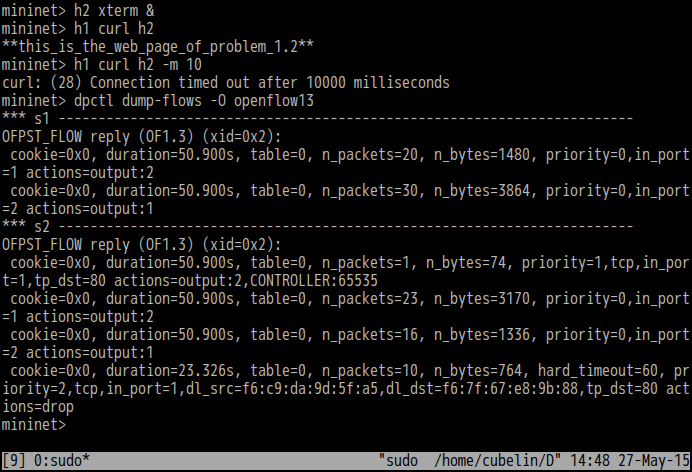
\includegraphics[width=.618\textwidth]{fig/1_2-2.png}
\caption{检查流表}\label{fig:Q1_2-2}
\end{figure}

5. 等待 60 秒,多次执行 \code{h1 curl h2},均能得到如下正常返回
\begin{center}
**this\_is\_the\_web\_page\_of\_problem\_1.2**
\end{center}
此时再检查流表,发现第 4 步时新增的流表已经过期。结果见\autoref{fig:Q1_2-3}

\begin{figure}[!h]
\centering
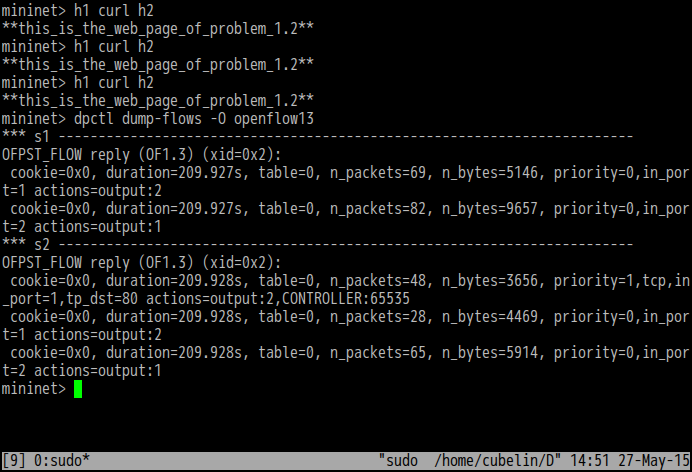
\includegraphics[width=.618\textwidth]{fig/1_2-3.png}
\caption{流表过期}\label{fig:Q1_2-3}
\end{figure}

\myparagraph{实验结果}

利用 Ryu Controller 提供的 Python API,自动化实现问题要求。

\clearpage

\section{第二题:提高题}\label{sec:Q2}
\subsection{第1小题:代理访问}\label{sec:Q2_1}

\begin{figure}[!h]
\centering
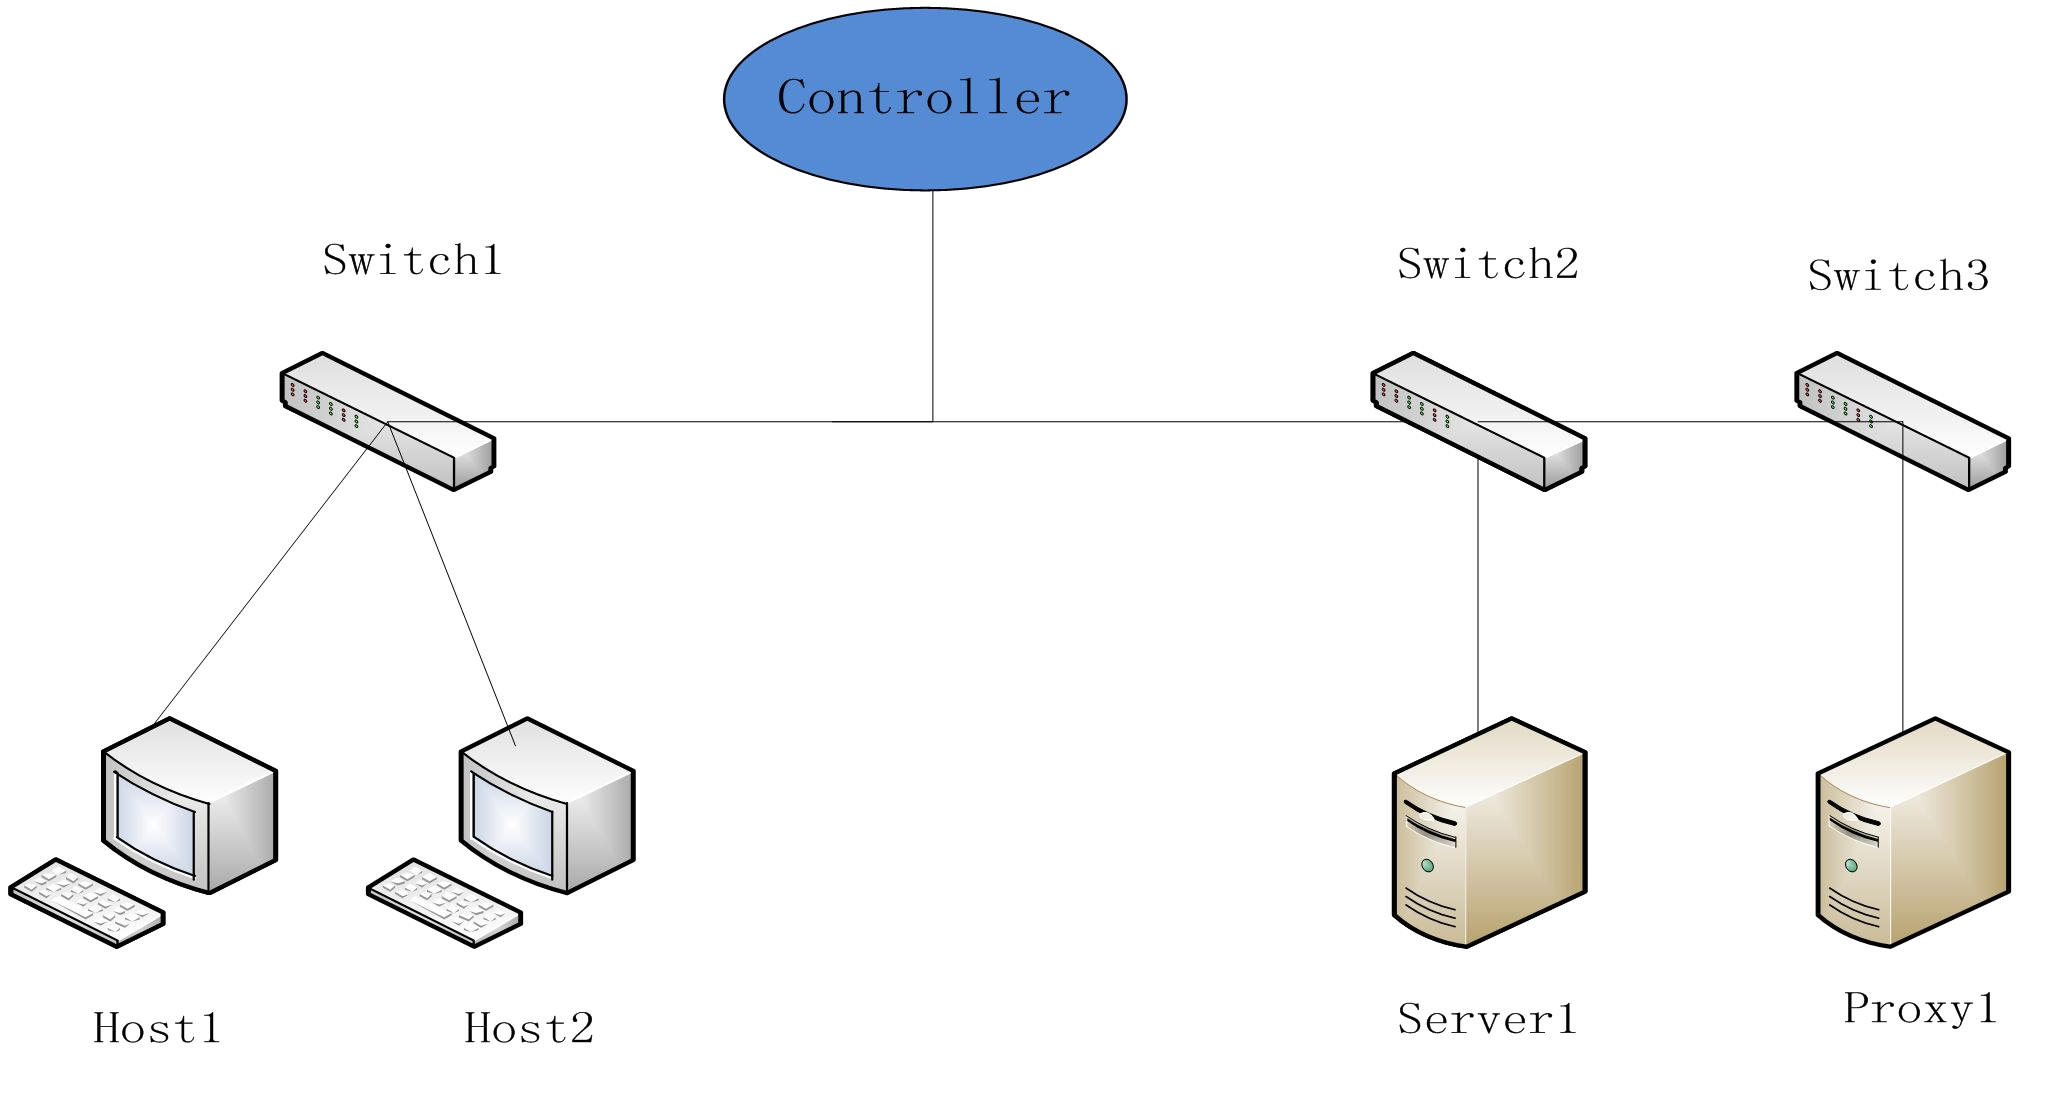
\includegraphics[width=.618\textwidth]{fig/2_1-0.png}
\caption{第二题第1小题:代理访问}\label{fig:Q2_1-0}
\end{figure}

\myparagraph{网络环境要求}

设有两台 PC 机(Host1,Host2),一台 Web 服务器(Server1)提供简单的静态网页访问服务,一台代理服务器(Proxy1)和 Web 服务器提供同样的服务,两
台服务器所显示的网页大致相同,但要有显著差别,可以是不同的网页内容或者不同颜色,能够区分彼此即可,如图 3 所示。(PC 机、Web 服务器、代理服务器、交换机、控制器可以选择物理设备或者虚拟设备实现)

\myparagraph{操作要求}

1.Web 服务器是 Host1 和 Host2 都可以访问的,而代理服务器是只有代理用户才可以使用。

2 可以设置 Host1 或 Host2 为代理用户,可以直接从代理服务器访问到网页。

\begin{figure}[!h]
\centering
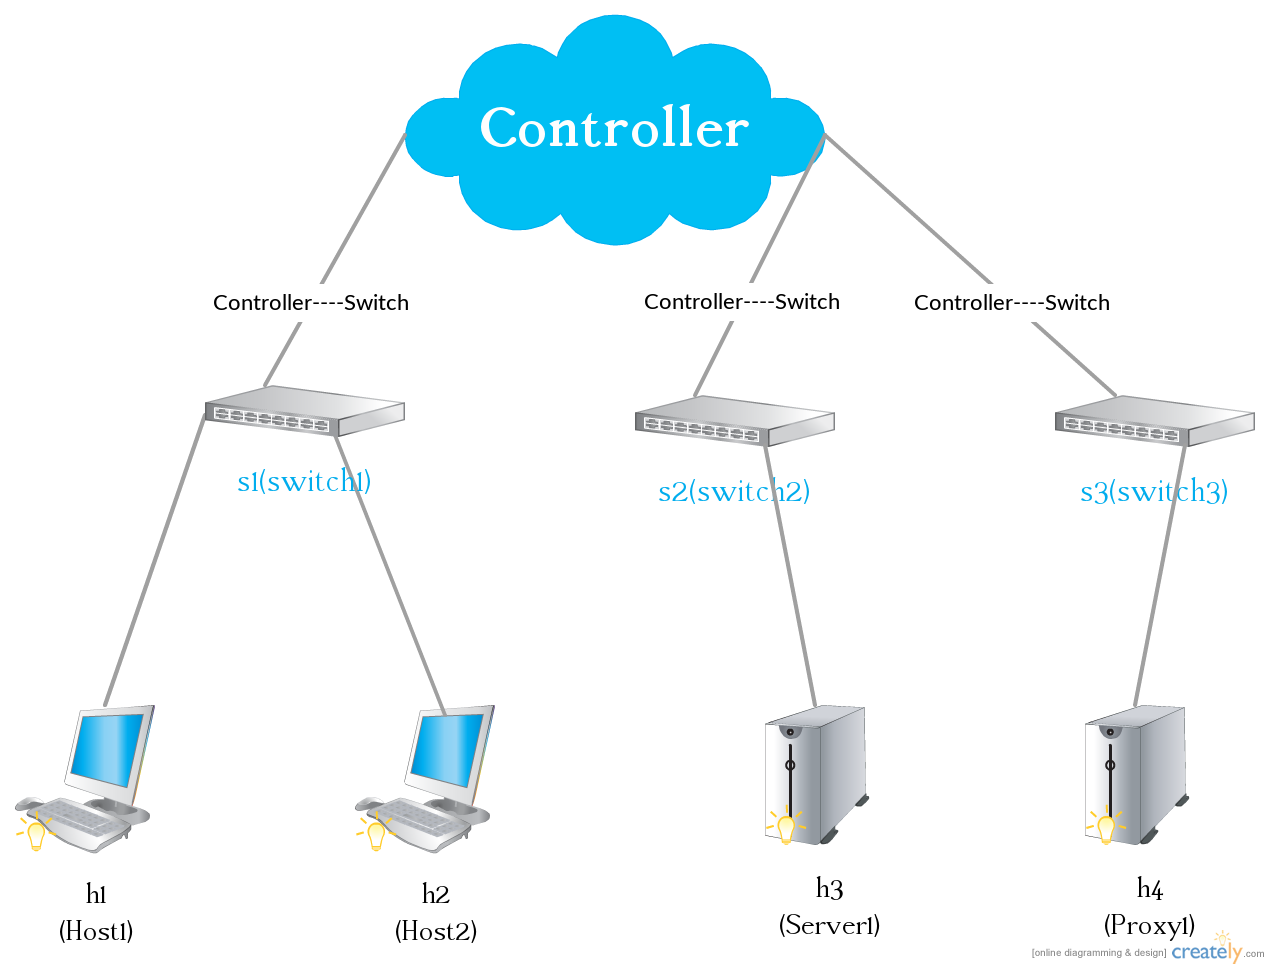
\includegraphics[width=.618\textwidth]{fig/2_1-4.png}
\caption{拓扑图}\label{fig:Q2_1-4}
\end{figure}

\myparagraph{方法描述}

拓扑图见\autoref{fig:Q2_1-4}。为了一般化,本题同样用 Ryu Controller Python API 实现。采用 Ryu 内置的 simple\_switch\_13 简单处理路由。编写第三方 Ryu Controller App,在交换机 s3 连接 Controller 时为其添加默认流表,丢弃所有来自 h2 并且发往 h4 的数据包。

\myparagraph{实验步骤}

1. 进入附件 2.1 目录,执行如下命令,其中 setup\_network.py 用于搭建虚拟网络环境,执行该脚本需要 root 权限。2\_1.py 是我们编写的 Ryu Controller App。

\begin{lstlisting}
python2 setup_network.py
ryu-manager 2_1.py ryu.app.simple_switch_13
\end{lstlisting}

交换机连接 Controller 后,会往 Controller 发送 Feature message。此时 Ryu 的 simple\_switch\_13 和 2\_1.py 中注册的回调都会被调用。2\_1.py 中往 s3 交换机添加流表的如下代码将会发挥作用。

\begin{lstlisting}[language=python]
...
    @set_ev_cls(ofp_event.EventOFPSwitchFeatures, CONFIG_DISPATCHER)
    def switch_feature_handler(self, ev):
        datapath = ev.msg.datapath
        parser = datapath.ofproto_parser
        dpid = datapath.id

        print 'Switch s%d connected.' % dpid
        if dpid == 3:
            match = parser.OFPMatch(in_port=1,
                                    eth_src=self.h2_mac, eth_dst=self.h4_mac)
            actions = []  # Drop
            # Flow entry:
            # table=0, priority=65535,in_port=1,dl_src=00:00:00:00:00:02,
            # dl_dst=00:00:00:00:00:04
            # actions=drop
            self.add_flow(datapath, 65535, match, actions)

...
\end{lstlisting}

2. 在 mininet CLI 中检查网络环境,输出流表如\autoref{fig:Q2_1-1},其中
\begin{center}
priority=65535,in\_port=1,dl\_src=00:00:00:00:00:02,dl\_dst=00:00:00:00:00:04 actions=drop
\end{center}

为 2\_1.py 为交换机 s3 添加的默认流表。

3. 在 mininet CLI 中执行 pingall,检查网络环境,结果如\autoref{fig:Q2_1-2},simple\_switch\_13 添加了多个流表保证网络通信。只有 h2 与 h4 互相无法 ping 通。

4. 搭建 Web 服务器。先在 mininet CLI 中执行 \code{h3 xterm \&}, 在打开的 xterm 中执行 \code{cd web \&\& python -m SimpleHTTPServer 80},再在 mininet CLI 中执行 \code{h4 xterm \&}, 在打开的 xterm 中执行 \code{cd proxy \&\& python -m SimpleHTTPServer 80},至此,Web Server 和 Web Proxy Server 搭建完毕。

5. 回到 mininet CLI 分别执行如下命令,得到输出如\autoref{fig:Q2_1-3},说明只有 h2 无法访问 h4(proxy)。

\begin{lstlisting}
h1 curl h3 -m 10
h1 curl h4 -m 10
h2 curl h3 -m 10
h2 curl h4 -m 10
\end{lstlisting}

\global\csname @topnum\endcsname 0 % prevent figures breaking lstlisting

\begin{figure}[!h]
\centering
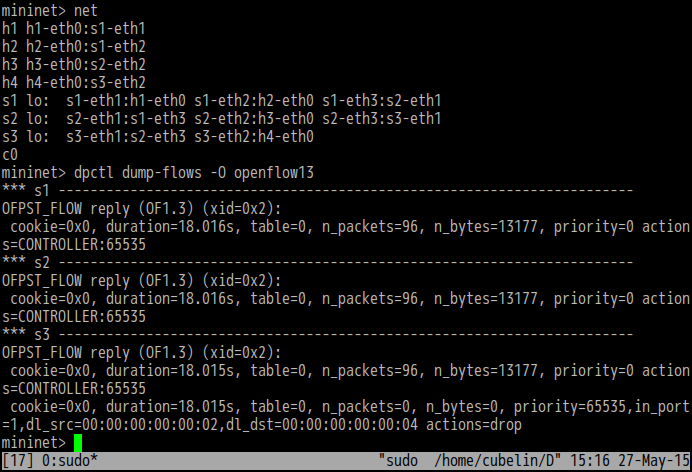
\includegraphics[width=.618\textwidth]{fig/2_1-1.png}
\caption{输出流表}\label{fig:Q2_1-1}
\end{figure}

\begin{figure}[!h]
\centering
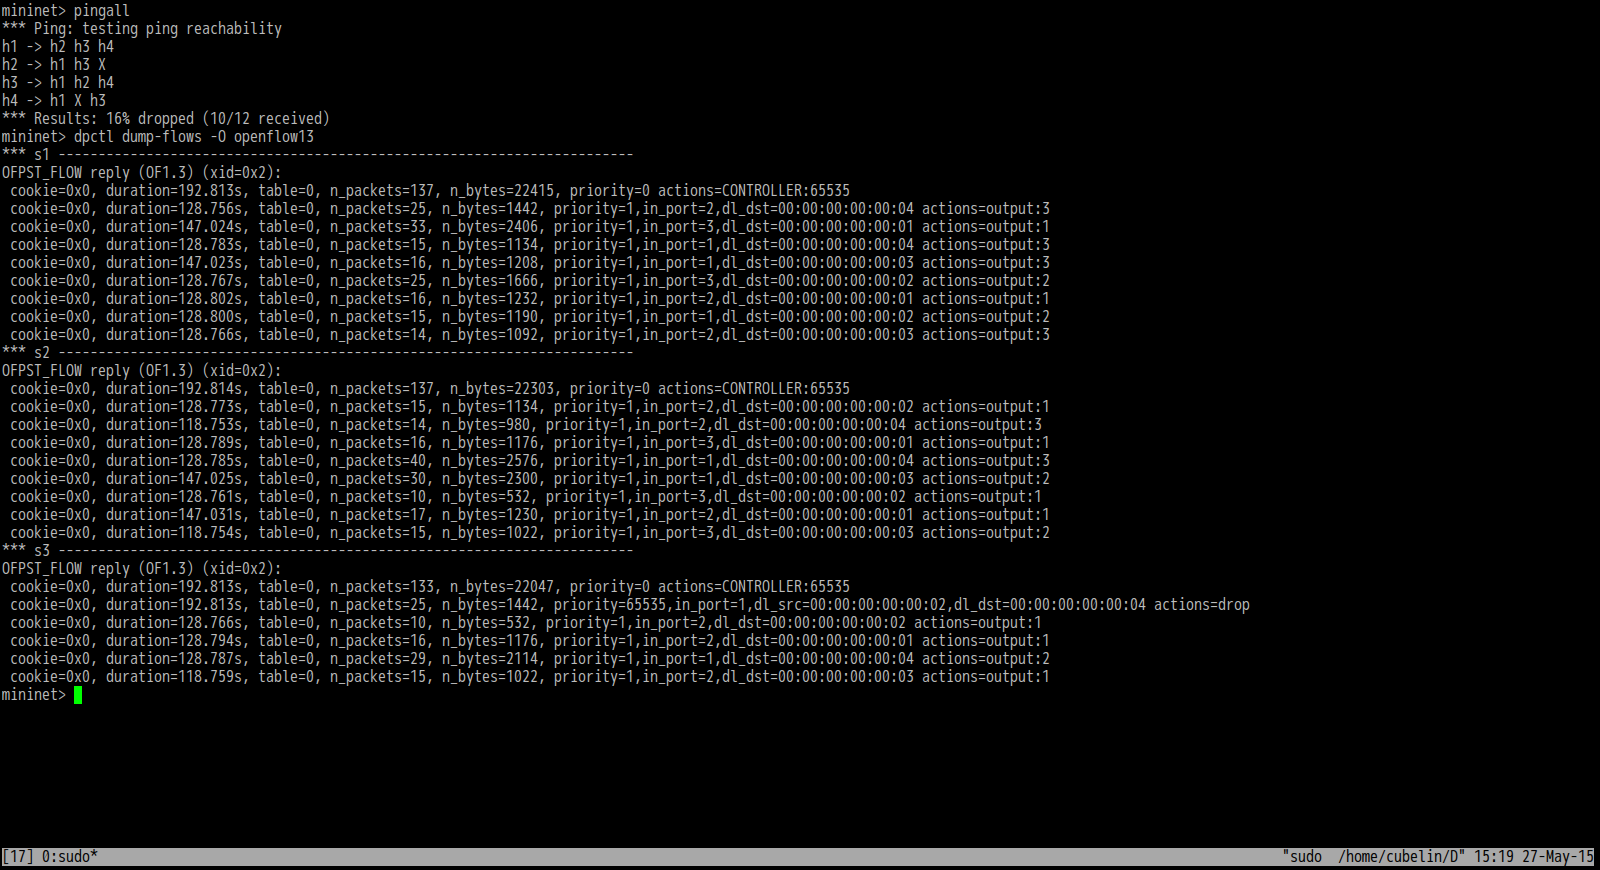
\includegraphics[width=\textwidth]{fig/2_1-2.png}
\caption{pingall结果与流表变化}\label{fig:Q2_1-2}
\end{figure}


\myparagraph{实验结果}

利用 Ryu Controller 提供的 Python API,自动化实现问题要求。

\begin{figure}[!h]
\centering
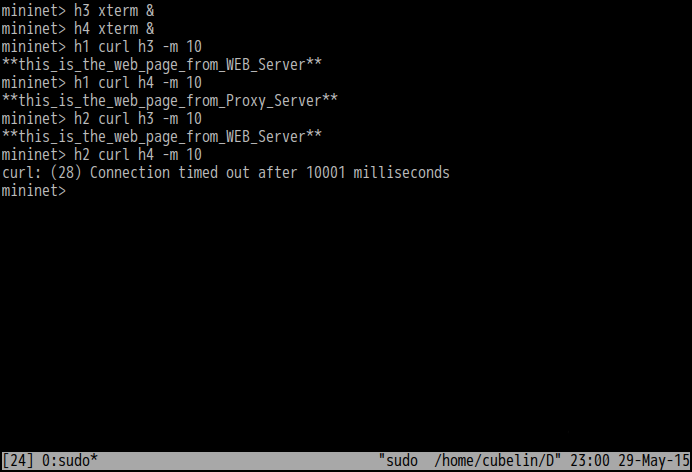
\includegraphics[width=.618\textwidth]{fig/2_1-3.png}
\caption{h1, h2 分别请求 h3, h4 网页的结果}\label{fig:Q2_1-3}
\end{figure}

\clearpage

\subsection{第2小题:流表管理}\label{sec:Q2_2}

\begin{figure}[!h]
\centering
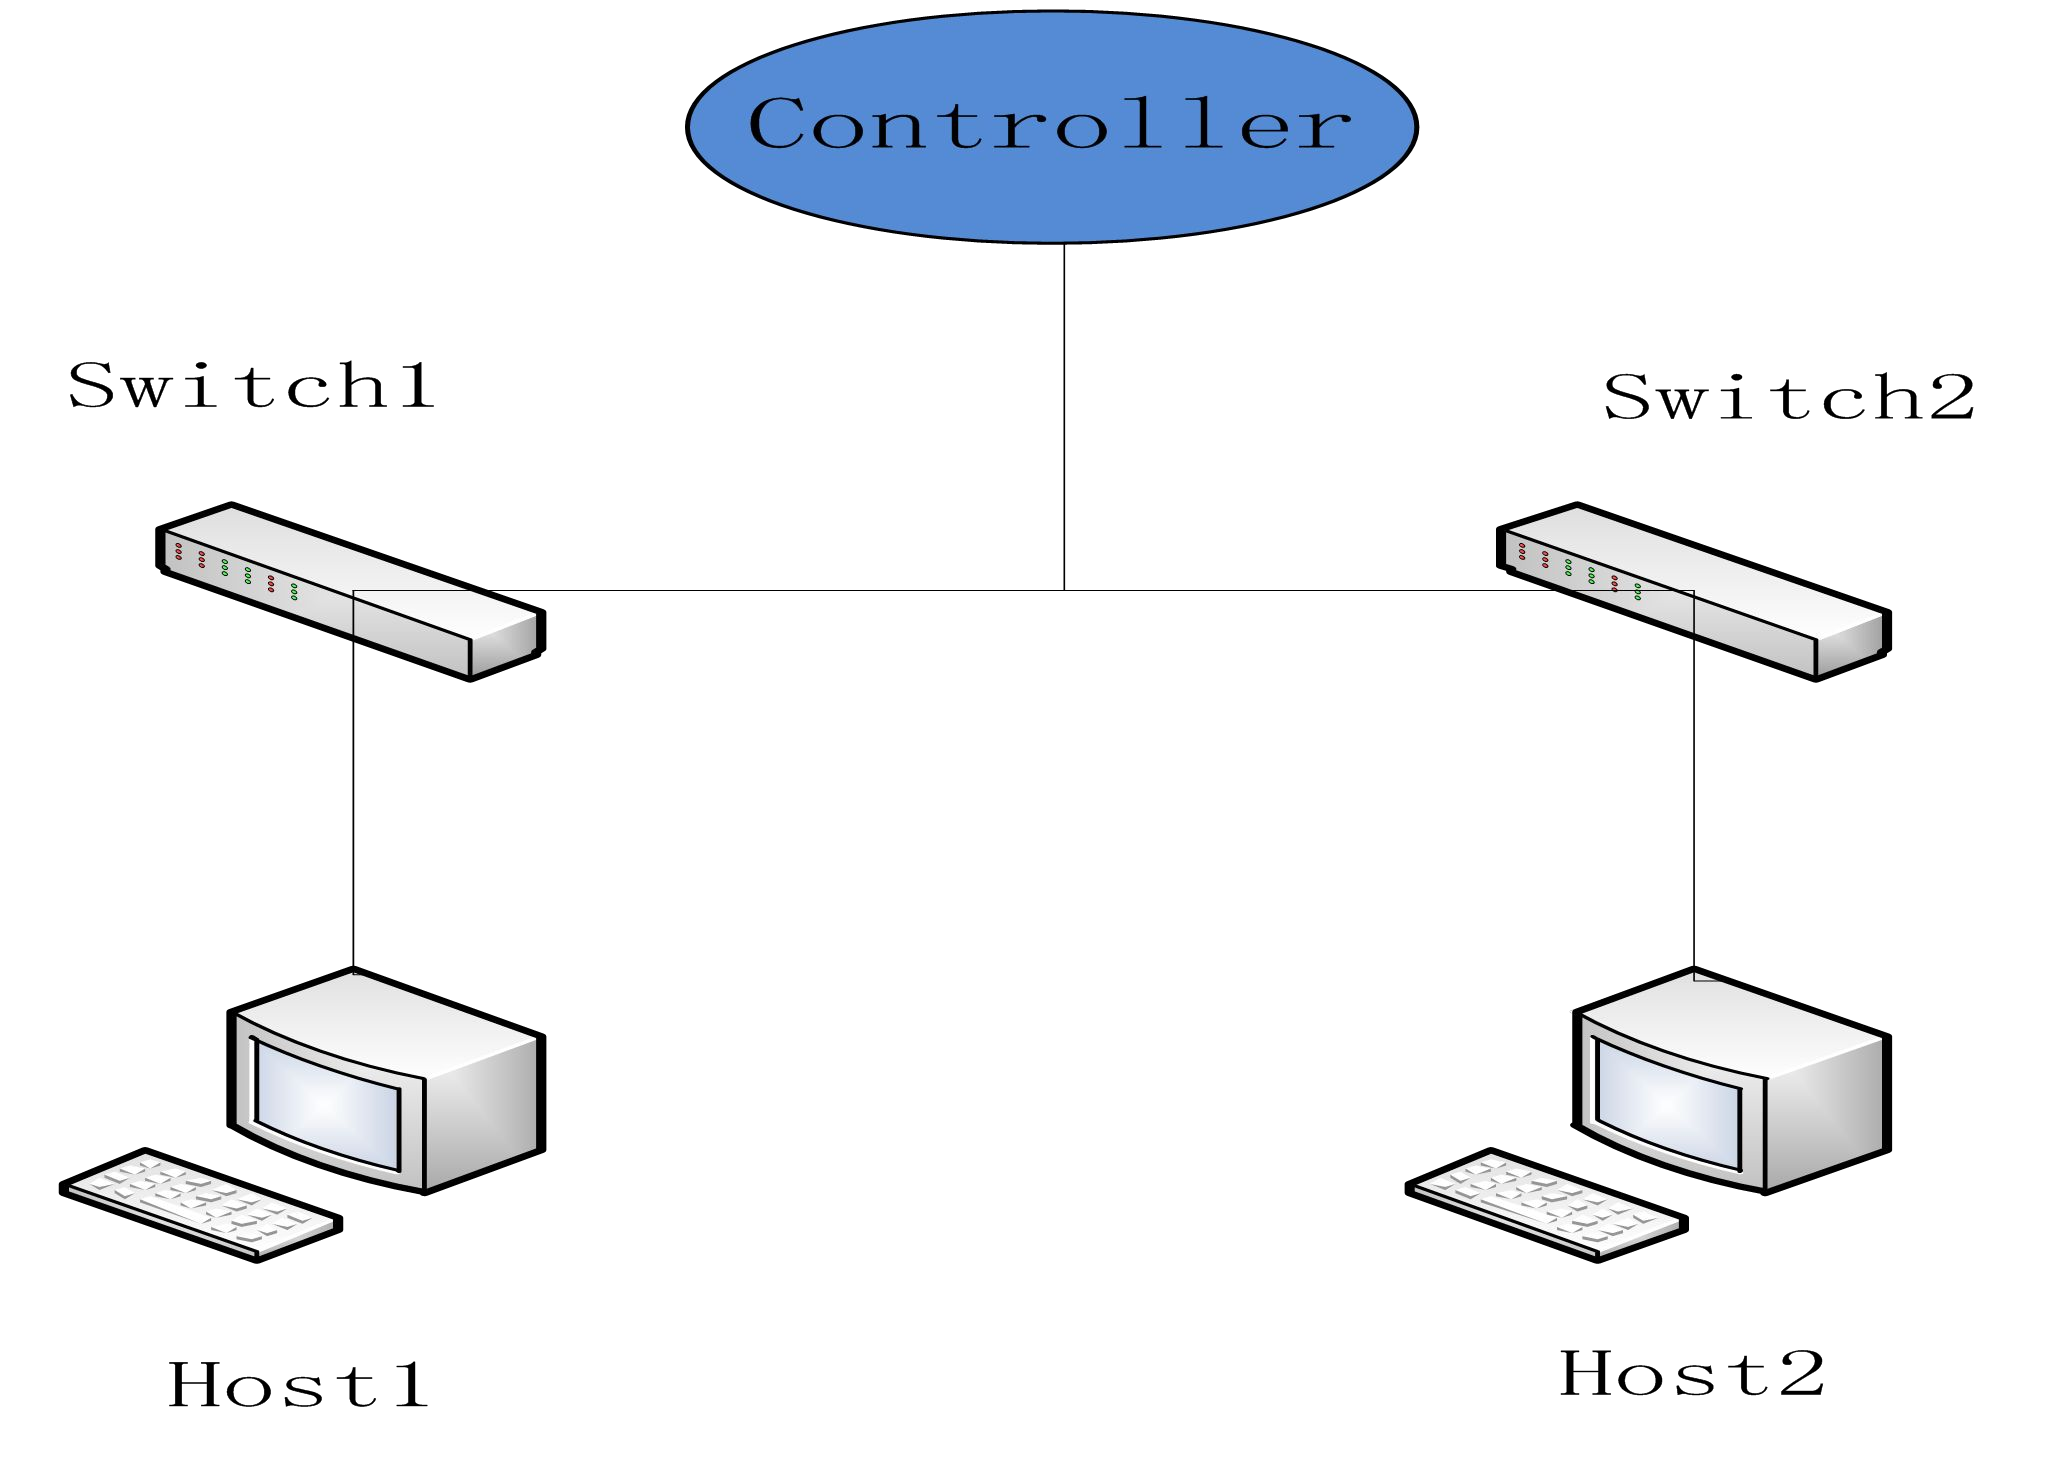
\includegraphics[width=.618\textwidth]{fig/2_2-0.png}
\caption{第二题第2小题:流表管理}\label{fig:Q2_2-0}
\end{figure}

\myparagraph{网络环境要求}

设有若干台 PC 机(Host1,Host2),若干台交换机(Switch1,Switch2),如图 4所示(作为示例拓扑,实际拓扑可自由选择)。(PC 机、交换机、控制器可以选择物理设备或者虚拟设备实现)

\myparagraph{操作要求}

利用控制器提供的 API(例如 REST API),开发一个网络及流表管理工具(客户端,网页端均可)。管理工具可以显示网络拓扑结构,查看流表,增加流表,删除流表。

\myparagraph{方法描述}

基于 Ryu 提供的北向接口开源实现,添加了少量独立开发的北向接口作为管理工具与 Controller 交互的接口,封装实现网络及流表的管理后台,前端使用 d3.js 绘制拓扑结构,并使用 Bootstrap 框架构建网页端。

\myparagraph{实验步骤}

1. 进入附件 2.2 目录,执行如下代码运行管理工具后端。

\begin{lstlisting}
ryu-manager --observe-links ryu.app.ofctl_rest rest_topology.py simple_switch_13.py
python wrapper.py
\end{lstlisting}

此时便可以通过 \url{http://localhost:8000/static/index.html} 预览管理工具,但是在交换机连接 Controller 之前,网页端不会显示任何相关信息。

补充说明:为了支持在网络拓扑中显示主机,我们对 Ryu 提供的 rest\_topology.py 进行了简单的修改,通过监测网络中通过交换机的 ARP 包和 IPv4 包,维护一个主机的状态表,并在前端请求拓扑结构时返回。 我们还对 simple\_switch\_13.py 进行了修改,让其添加的路由 flow entry 拥有过期时间,便于 Controller 及时更新状态表。

2. 执行如下命令,用 mininet 构建虚拟网络环境,并连接 Controller.
\begin{lstlisting}
sudo mn --switch ovsk --topo tree,3,fanout=3 --controller remote,ip=127.0.0.1
\end{lstlisting}

3. 在 mininet CLI 中执行 \code{pingall},让 Controller 发现主机。

4. 访问 \url{http://localhost:8000/static/index.html} ,可以看到拓扑图以及所有交换机上的流表。之后如若交换机甚至是整个网络环境断开重新连接,只需要点击两个 Refresh 按钮刷新即可。

网络拓扑部分显示如\autoref{fig:Q2_2-1}。

\begin{figure}[!h]
\centering
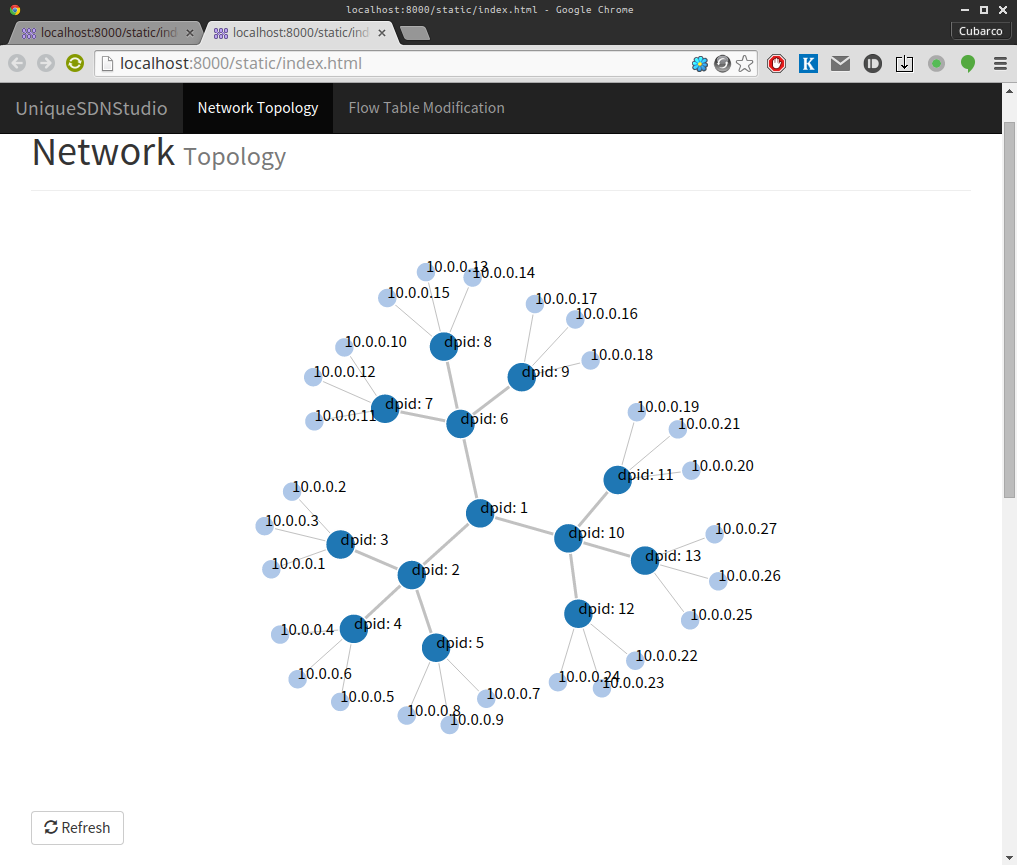
\includegraphics[width=.7\textwidth]{fig/2_2-1.png}
\caption{网络拓扑图}\label{fig:Q2_2-1}
\end{figure}

流表部分显示如\autoref{fig:Q2_2-2}。

\begin{figure}[!h]
\centering
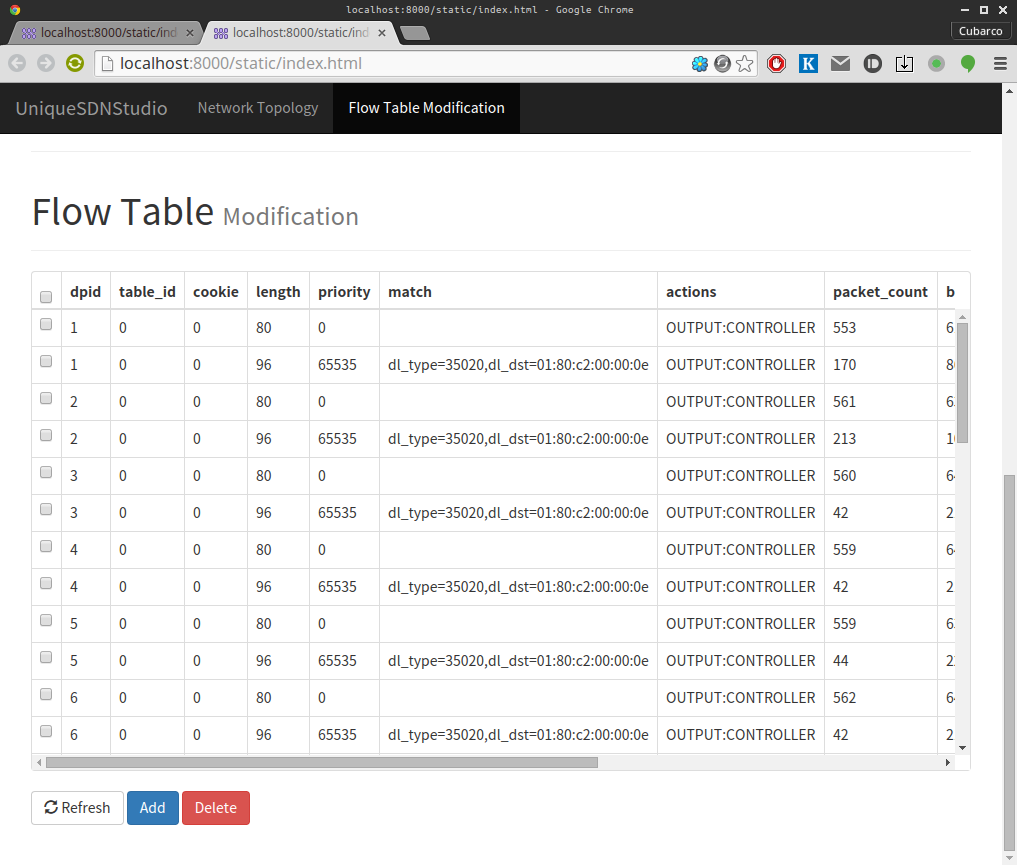
\includegraphics[width=.7\textwidth]{fig/2_2-2.png}
\caption{流表管理}\label{fig:Q2_2-2}
\end{figure}

5. 预设若 6 分钟无某主机的包通过交换机,将会从状态表中删除该主机的记录。6 分钟后点击 Refresh 按钮,网络拓扑如\autoref{fig:Q2_2-3}。

\begin{figure}[!h]
\centering
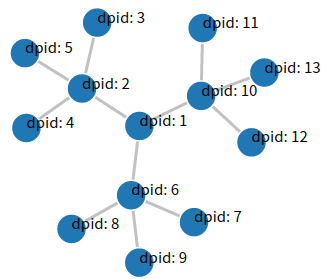
\includegraphics[width=.4\textwidth]{fig/2_2-3.png}
\caption{6 分钟后的网络拓扑图}\label{fig:Q2_2-3}
\end{figure}

6. 测试删除 flow entry 的功能:勾选相应的 flow entry ,点击 Delete 按钮,确认后,相应的 flow entry 将会被删除,并从网页中消失,过程见\autoref{fig:Q2_2-S1}。

注意: 选择相应 flow entry 之前务必点击 Refresh 按钮刷新。

\begin{figure}[!h]
\centering
  \begin{subfigure}[b]{.48\textwidth}
  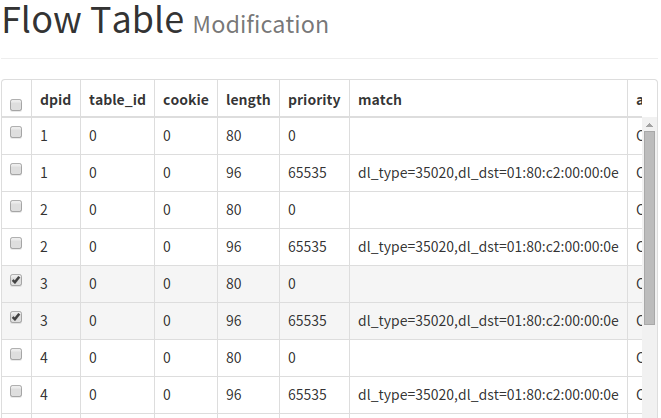
\includegraphics[width=\textwidth]{fig/2_2-4}
  \caption{选中与 s3 交换机相关的 flow entry}\label{fig:Q2_2-4}
  \end{subfigure}
  ~
  \begin{subfigure}[b]{.48\textwidth}
  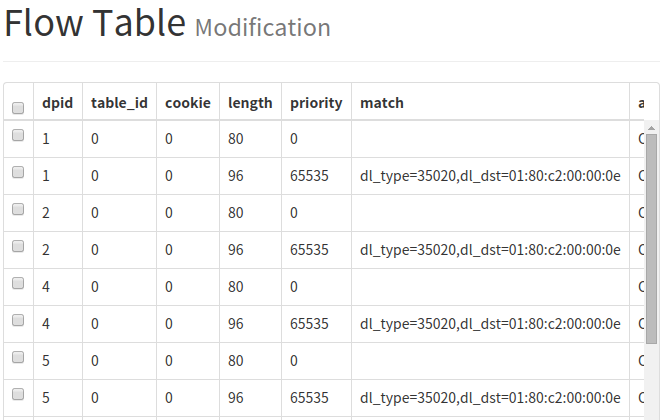
\includegraphics[width=\textwidth]{fig/2_2-5}
  \caption{删除后}\label{fig:Q2_2-5}
  \end{subfigure}
\caption{删除流表操作}\label{fig:Q2_2-S1}
\end{figure}

从 \autoref{fig:Q2_2-1} 可以看到,主机 h1 直接接在 s3 交换机上,所以在 mininet CLI 中执行如下命令:
\begin{lstlisting}
h1 ping h4
h1 ping h5
h4 ping h5
\end{lstlisting}

结果如\autoref{fig:Q2_2-6}所示,h1 无法与外界通信,而 s1 交换机外的环境通信正常,说明 flow entry 成功删除。

\begin{figure}[!h]
\centering
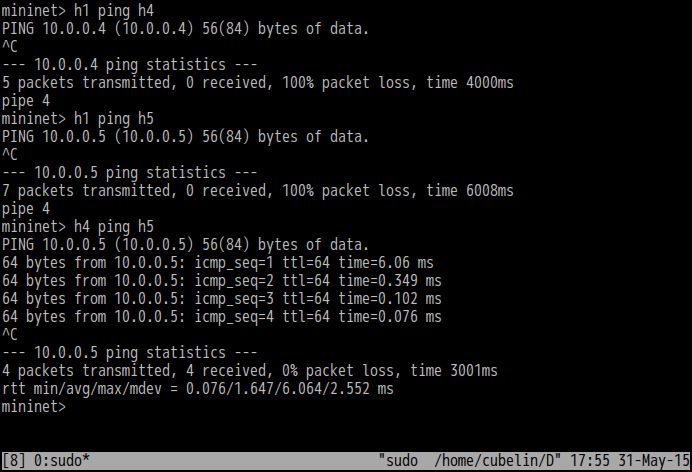
\includegraphics[width=.618\textwidth]{fig/2_2-6.png}
\caption{ping 结果图}\label{fig:Q2_2-6}
\end{figure}

7. 测试添加 flow entry 的功能:在上述实验步骤的前提下,点击 Add 按钮,如\autoref{fig:Q2_2-7}填写相关信息(match 项填空格表示匹配所有),output 端口填 \code{4294967293} 表示发给 Controller. 再次点击 Add 按钮添加,如果添加成功将在网页上显示新的 flow entry.

\begin{figure}[!h]
\centering
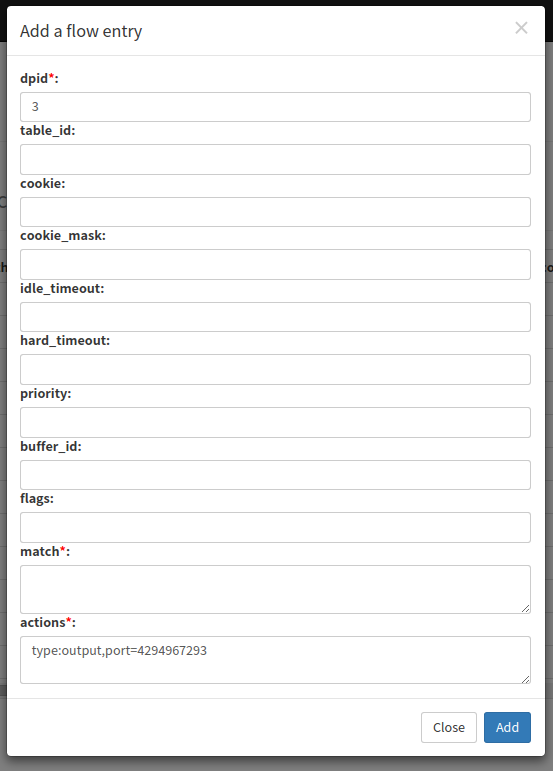
\includegraphics[width=.618\textwidth]{fig/2_2-7.png}
\caption{添加 flow entry}\label{fig:Q2_2-7}
\end{figure}

在 mininet CLI 中执行 \code{pingall},发现 h1 能 ping 通所有主机,表示 flow entry添加成功,结果见\autoref{fig:Q2_2-8}。

\begin{figure}[!h]
\centering
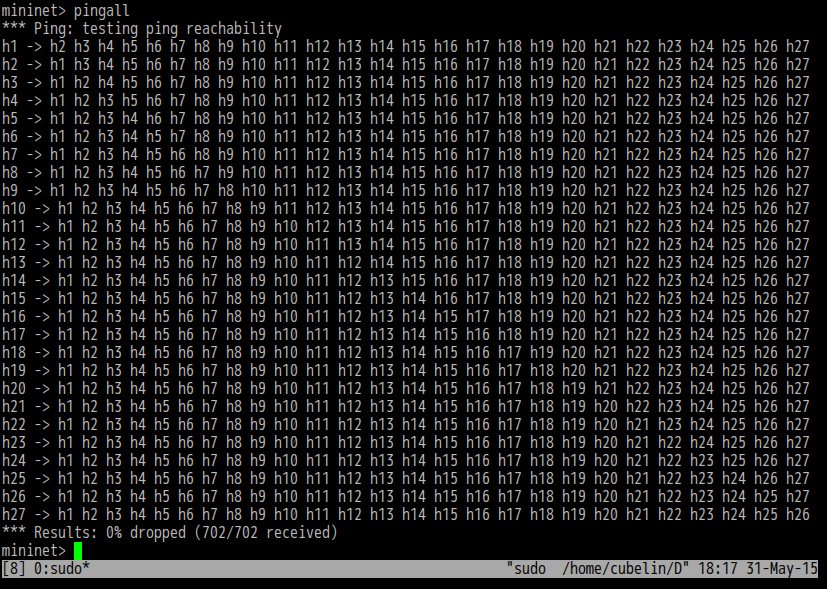
\includegraphics[width=.5\textwidth]{fig/2_2-8.png}
\caption{添加 flow entry 后 pingall}\label{fig:Q2_2-8}
\end{figure}

\myparagraph{实验结果}

显示网络拓扑图,查看流表,增加流表,删除流表等功能测试成功。

\clearpage

\section{第三题:设计题}\label{sec:Q3}

\myparagraph{选题背景}

随着互联网逐渐渗透到人们生活的每一个角落,人们的生活也变得越来越便利了。但是网络也是一把双刃剑。在它越来越多的控制人们的生活的同时,它不安全的一面也渐渐暴露出来。网络攻击随处可见,造成了难以估计的损失。对于一般民众而言,恶意网站、钓鱼链接是对他们数据、财产安全最大的威胁,需要小心应对。

\myparagraph{设计细节}
\begin{figure}[!h]
\centering
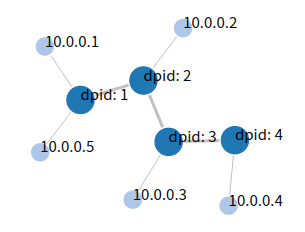
\includegraphics[width=.5\textwidth]{fig/3_0-0}
\caption{设计题网络拓扑图}\label{fig:Q3-0-0}
\end{figure}

如\autoref{fig:Q3-0-0}所示,网络为线性拓扑,共4个host,分别与4个交换机相连(s1,s2,s3,s4)。这四个交换机互相之间也有连接。为了使hosts可以访问外网,故使用了nat参数使得本机桥接到 mininet 虚拟网络环境内,作为 h5 连接在s1上。h1,h2的网关是h3。将controller上的dnsserver设置为h4的mac地址,将dns请求全部劫持到h4上。h4上运行fakedns.py来处理所有dns请求。

设计与实现方案:controller 运行一个经过修改的交换机算法。对于除dns包以外的数据包按正常的交换机进行学习和转发,对于dns查询数据包则将目的mac地址强制设为dnsserver然后再进行交换算法。这样就可以将dns查询报文劫持到h4上。而h4上运行的fakedns将过滤出所有dns包并检查其查询的网址是否在黑名单中,若在黑名单中则不进行响应,否则将该数据包正常送往网关,然后将回应数据包转回来源host。

\myparagraph{实验步骤}
\begin{figure}[!h]
\centering
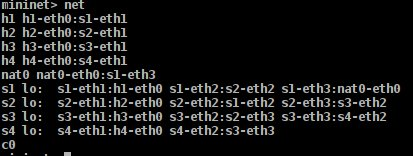
\includegraphics[width=.5\textwidth]{fig/3_0}
\caption{创建网络拓扑}\label{fig:Q3-0}
\end{figure}

1. 执行如下命令创建网络拓扑,得到如\autoref{fig:Q3-0}的网络结构。
\begin{lstlisting}
mn --controller=remote --topo=linear,4 --nat
\end{lstlisting}

2. 进入附件的目录 3,执行如下命令运行 Controller:
\begin{lstlisting}
ryu-manager 3.py
\end{lstlisting}

3. 在 mininet CLI 中执行 \code{pingall},结果如\autoref{fig:Q3-5},说明通信正常。

\begin{figure}[!h]
\centering
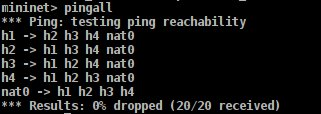
\includegraphics[width=.5\textwidth]{fig/3_5}
\caption{检查网络环境}\label{fig:Q3-5}
\end{figure}

4. 检查各主机网络设置,结果见\autoref{fig:Q3-1},\autoref{fig:Q3-3},\autoref{fig:Q3-4}。在 mininet CLI 中执行\code{h1 ip r replace default via 10.0.0.3}配置h1的默认路由,并执行 \code{h1 ip r} 检查结果,见 \autoref{fig:Q3-2}。
\begin{figure}[!h]
\centering
  \begin{subfigure}[b]{0.48\textwidth}
  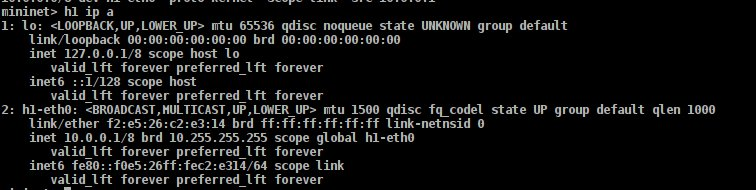
\includegraphics[width=\textwidth]{fig/3_1}
  \caption{h1 网络设置}\label{fig:Q3-1}
  \end{subfigure}
  ~
  \begin{subfigure}[b]{0.48\textwidth}
  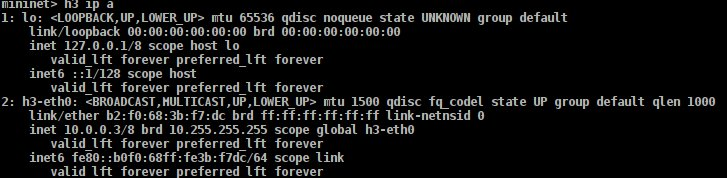
\includegraphics[width=\textwidth]{fig/3_3}
  \caption{h3 网络设置}\label{fig:Q3-3}
  \end{subfigure}
  ~
  \begin{subfigure}[b]{0.48\textwidth}
  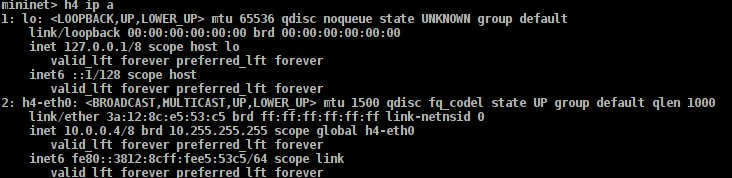
\includegraphics[width=\textwidth]{fig/3_4}
  \caption{h4 网络设置}\label{fig:Q3-4}
  \end{subfigure}
  ~
  \begin{subfigure}[b]{0.48\textwidth}
  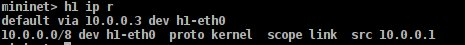
\includegraphics[width=\textwidth]{fig/3_2}
  \caption{h1 的路由表配置}\label{fig:Q3-2}
  \end{subfigure}
\caption{各主机网络设置}\label{fig:Q3-S1}
\end{figure}

5. 在 h4 上运行fakedns.py,配置文件中默认屏蔽baidu.*,如\autoref{fig:Q3-6}
\begin{figure}[!h]
\centering
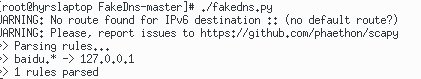
\includegraphics[width=.618\textwidth]{fig/3_6}
\caption{运行 fakedns.py}\label{fig:Q3-6}
\end{figure}

6. 在 mininet CLI 中执行 \code{h1 nslookup www.google.com},结果如\autoref{fig:Q3-8},正常得到返回。
fakedns.py 的日志见\autoref{fig:Q3-9}。
\begin{figure}[!h]
\centering
  \begin{subfigure}[b]{0.48\textwidth}
  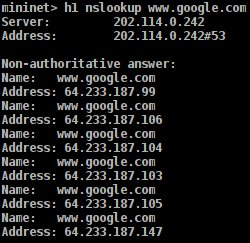
\includegraphics[width=\textwidth]{fig/3_8}
  \caption{查询 www.google.com 的 DNS 记录}\label{fig:Q3-8}
  \end{subfigure}
  ~
  \begin{subfigure}[b]{0.48\textwidth}
  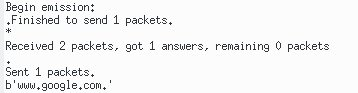
\includegraphics[width=\textwidth]{fig/3_9}
  \caption{fakedns.py 的日志}\label{fig:Q3-9}
  \end{subfigure}
\caption{www.baidu.com 的 DNS 记录查询情况}\label{fig:Q3-S2}
\end{figure}

7. 在 mininet CLI 中执行 \code{h1 nslookup www.baidu.com},结果如\autoref{fig:Q3-11},查询超时。fakedns.py 的日志见\autoref{fig:Q3-12}。
\begin{figure}[!h]
\centering
  \begin{subfigure}[b]{0.48\textwidth}
  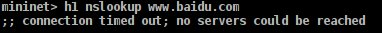
\includegraphics[width=\textwidth]{fig/3_11}
  \caption{查询 www.baidu.com 的 DNS 记录}\label{fig:Q3-11}
  \end{subfigure}
  ~
  \begin{subfigure}[b]{0.48\textwidth}
  
\includegraphics[width=\textwidth]{fig/3_12}
  \caption{fakedns.py 的日志}\label{fig:Q3-12}
  \end{subfigure}
\caption{www.baidu.com 的 DNS 记录查询情况}\label{fig:Q3-S3}
\end{figure}

\myparagraph{试验结果}

此方案可以成功阻止对恶意网址的dns查询,进而保护用户安全
\clearpage

\backmatter

%\begin{ack}
%致谢正文。
%\end{ack}

\bibliography{ref}

%\appendix

%\begin{publications}
    %\item 论文1
    %\item 论文2
%\end{publications}

%\chapter{这是一个附录}\label{appendix:2}
%附录正文。


\end{document}
\endinput
%%
%% End of file `hustreport-zh-example.tex'.
